\chapter{Eksperymenty\label{chap:eksperymenty}}

\section{Wprowadzenie}
W niniejszym rozdziale zostały zebrane wyniki testów dla algorytmów, których opisy zostały umieszczone w rozdziałach~\ref{chap:teoria} oraz~\ref{chap:algorytm}. Implementacja tychże algorytmów została wykonana w technologiach opisanych w rozdziale~\ref{chap:technologie}.

Testy zostały przeprowadzone na laptopie ASUS U36JC wyposażonym w procesor Intel Core i5 460M/480M 2.66 GHz oraz kartę graficzną NVIDIA GeForce 310M with 1GB DDR3 VRAM z systemem oparacyjnym był Windows 7 Home Professional. Co ważne testy dla każdego typu algorytmu oraz parametrów wejściowych wykonane zostały w dwóch przypadkach - na zasilaniu z włączonym trybem \emph{pełnej mocy} oraz na baterii, z włączonym trybem \emph{oszczędzania energii}. Dzięki temu drugiemu emulowana była sytuacja, gdy komputer był wyposażony w wyższej klasy kartę graficzną niż model, na którym przeprowadzone zostały testy - ponieważ w trybie oszczędzania energii to moc procesora była ograniczana, natomiast nic się nie działo z parametrami pracy dla karty graficznej.

Dane testowe zostały pobrane ze strony \url{Htp://kdd.ics.uci.edu/databases/msweb/msweb.Hml} Plik zawiera informacje, jakie strony serwisu \url{www.microsoft.com} zostały odwiedzone przez poszczególnych użytkowników w tygodniowym oknie czasowym na przestrzeni lutego 1998 roku. W tabeli~\ref{msweb:desc} zebrane zostały podstawowe informacje na temat danych testowych.

\begin{table}
	\centering
	\begin{tabular}{l|l}
	Liczba transakcji & 32711 \\
	Elementów & 294 \\ 
	Rozmiar pliku & $1390$KB ($1.35$MB)\\
	\end{tabular}
	\caption{Podstawowe informacje o danych testowych MSWebData\label{msweb:desc}}
\end{table}

\section{Wyniki eksperymentów}
\subsection{Wyniki pomiarów poszczególnych implementacji algorytmów}

W części tej zostaną przedstawione wyniki testów dla poszczególnych implementacji przedstawionych wcześniej algorytmów. Wykonanych został szereg testów aby uwiarygodnić jak najbardziej wyniki, a także wykazać wpływ parametrów wejściowych (minsup, minconf) na czas wykonywania się algorytmu.

%%%%%%%%%%%%%%%%%%%%%%%%%%%%%%%%%%%%%%%%%
%%%%%%%%%%%%%%%%%%%%%%%%%%%%%%%%%%%%%%%%%
%%%%%%%%%%%%%%%%%%%%%%%%%%%%%%%%%%%%%%%%%
%%%%%%%%%%%%%%%%%%%%%%%%%%%%%%%%%%%%%%%%%
%%%%%%%%%%%%%%%%%%%%%%%%%%%%%%%%%%%%%%%%%

\subsubsection{Wyniki dla minsup = 0.2, minconf = 0.1}

\begin{figure}[H]
\centering
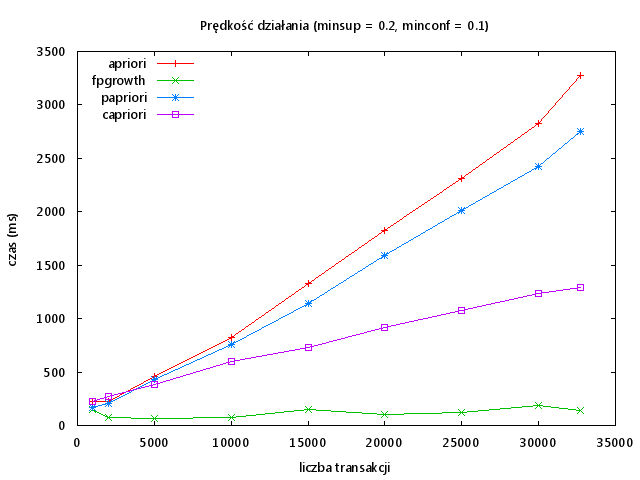
\includegraphics[width=1.1\textwidth]{figures/06/02_01.png}
\caption{Prędkość działania algorytmów\label{rys:02_01}}
\end{figure}

\begin{table}
	\centering
	\begin{tabular}{r|r|r|r|r}
	\textbf{l.trans} & \textbf{Apriori} & \textbf{FPGrowth} & \textbf{ParallelApriori} & \textbf{CudaApriori} \\ \hline
	$1000$ & $224$ & $146$ & $167$ & $221$ \\
	$2000$ & $224$ & $71$ & $202$ & $268$ \\
	$5000$ & $463$ & $70$ & $429$ & $388$ \\
	$10000$ & $825$ & $77$ & $758$ & $601$ \\
	$15000$ & $1330$ & $149$ & $1141$ & $726$ \\
	$20000$ & $1822$ & $102$ & $1594$ & $914$ \\
	$25000$ & $2315$ & $124$ & $2016$ & $1080$ \\
	$30000$ & $2823$ & $190$ & $2420$ & $1232$ \\
	$32711$ & $3274$ & $138$ & $2755$ & $1291$ \\
	\end{tabular}
	\caption{Czasy wykonania poszczególnych algorytmów [ms] (minsup = 0.2, minconf = 0.1)\label{tab:02_01}}
\end{table}

Rysunek~\ref{rys:02_01} przedstawia wykres czasów poszukiwania reguł asocjacyjnych przez poszczególne algorytmy. Poszczególne wartości zebrane zostały w tabeli~\ref{tab:02_01}. 

Jak łatwo zauważyć dla tego zbioru danych algorytm referencyjny, jakim jest FPGrowth poradził sobie znakomicie - czasy jego wykonywania były praktycznie pomijalne, co łatwo zauważyć porównując wynik dla $1000$ oraz $32711$, kiedy to dla mniejszej liczby transakcji algorytm działał dłużej. Takie wahania czasowe wynikają ze specyfiki budowy procesora oraz systemu operacyjnego, w którym poszczególne procesy są wywłaszczane przez inne procesy, co jest sytuacją niedeterministyczną i może, lecz nie musi się zdarzyć.

Interesujące obserwacje, zgodne z intuicją - przynoszą pozostałe 3 wykresy. Widać wyraźnie, że podstawowa implementacja algorytmu Apriori wypadła najgorzej z całej 3. Dla całego zbioru danych wejściowych czas wykonania algorytmu był o prawie $16\%$ gorszy od ParallelApriori oraz ponad $154\%$ wolniejszy od algorytmu CudaApriori. 

Algorytm ParallelApriori uplasował się mniej więcej po środku rankingu, jednakże bliżej mu do klasycznej wersji niż do wersji zrównoleglonej przy użyciu technologii CUDA. Ponieważ tylko niektóre elementy algorytmu zostały zrównoleglone nie można było oczekiwać $2$ krotnego przyspieszenia algorytmu, a tylko częściowe jego usprawnienie. Oczekiwanie to zostało spełnione, choć w tym miejscu należy zaznaczyć, że istnieje jeszcze przestrzeń, w której można popracować nad udoskonaleniem algorytmu - m.in. opracowując inne struktury danych, które będą mogły być lepiej wykorzystywane przez PLINQ.

Spośród trzech algorytmów klasy apriori, najwydajniejszym algorytmem jest algorytm CudaApriori, co podpowiadała intuicja jeszcze przed uruchomieniem testów wydajnościowych. Należy podkreślić, że algorytm ten dla zadanych parametrów wejściowych jest niemalże $3$ razy szybszy od klasycznej implementacji, a także ponad $2$ razy szybszy od wersji zrównoleglonej przy użyciu PLINQ.

\begin{figure}[H]
\centering
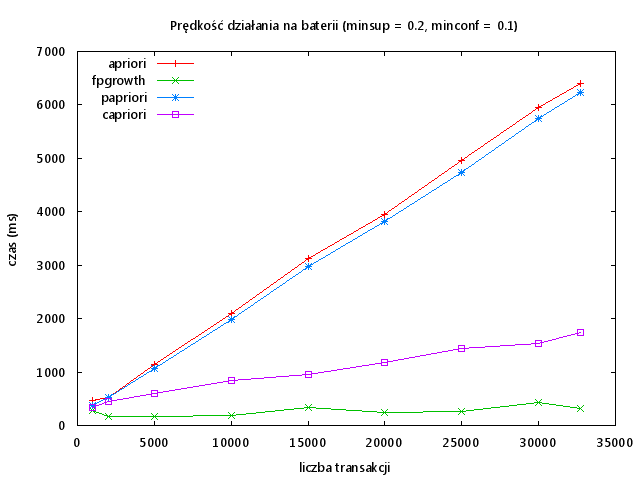
\includegraphics[width=1.1\textwidth]{figures/06/02_01_bat.png}
\caption{Prędkość działania algorytmów na baterii laptopa\label{rys:02_01_bat}}
\end{figure}

Rysunek~\ref{rys:02_01_bat} (na podstawie danych z tablicy~\ref{tab:02_01_bat}) przedstawia te same algorytmy, o których pisano wyżej, jednakże wykonywane w trybie oszczędzania baterii laptopa. Wyraźnie widać spadek wydajności implementacji algorytmów na CPU, w porównaniu do GPU.

Algorytm referencyjny po raz kolejny okazał się bezkonkurencyjny, jednakże również na jego przykładzie widać spadek wydajności spowodowany obniżeniem taktowania procesora.

W wyraźny sposób zmniejszyła się różnica pomiędzy implemntacjami algorytmu Apriori na CPU - wcześniej wynosiła około $16\%$, gdy podczas pracy na baterii wyniosła jedynie niecałe $3\%$. Wartość ta bierze się również z faktu obniżenia wydajności poszczególnych rdzeni, jak i wydajności całego układo - m.in. komunikacji pomiędzy rdzeniami.

Wydłużył się, jednak już nie tak znacznie, czas wykonywania CudaApriori. Nadal ma on przewagę nad Apriori (niemalże $270\%$) oraz ParallelApriori (niemalże $260\%$). Zastosowanie jeszcze lepszej karty graficznej do wykonywania testów algorytmu w CUDA pozwoliłoby osiągnąć jeszcze lepszy rezultat.

Pozostaje odpowiedzieć na pytanie, dlaczego zwiększył się czas odpowiedzi również dla CudaApriori. Wynika to z faktu, że część logiki biznesowej dla algorytmu została zaimplementowana klasycznie, przy użyciu procesora, a obniżenie jego wydajności wpływao bezpośrednio na algorytm, którego znaczna część wykonywała się równolegle, na jednostce graficznej.

\begin{table}
	\centering
	\begin{tabular}{r|r|r|r|r}
	\textbf{l.trans} & \textbf{Apriori} & \textbf{FPGrowth} & \textbf{ParallelApriori} & \textbf{CudaApriori}  \\ \hline
	$1000$ & $467$ & $281$ & $383$ & $339$ \\
	$2000$ & $526$ & $160$ & $531$ & $445$ \\
	$5000$ & $1140$ & $168$ & $1073$ & $592$ \\
	$10000$ & $2097$ & $181$ & $1986$ & $847$ \\
	$15000$ & $3127$ & $344$ & $2983$ & $951$ \\
	$20000$ & $3951$ & $242$ & $3811$ & $1183$ \\
	$25000$ & $4955$ & $254$ & $4741$ & $1436$ \\
	$30000$ & $5957$ & $431$ & $5750$ & $1527$ \\
	$32711$ & $6398$ & $319$ & $6233$ & $1734$ \\
	\end{tabular}
	\caption{Czasy wykonania poszczególnych algorytmów na baterii laptopa [ms] (minsup = 0.2, minconf = 0.1)\label{tab:02_01_bat}}
\end{table}

\begin{figure}[H]
\centering
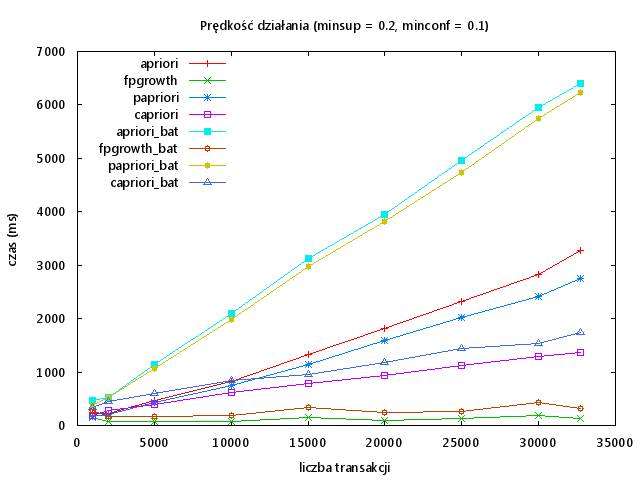
\includegraphics[width=1.1\textwidth]{figures/06/02_01_all.png}
\caption{Prędkość działania algorytmów w dwóch środowiskach uruchomieniowych\label{rys:02_01_all}}
\end{figure}

Rysunek~\ref{rys:02_01_all} prezentuje porównanie poszczególnych algorytmów w dwóch środowiskach uruchomieniowych. Potwierdza się fakt obniżenia wydajności poszczególnych algorytmów, wynikający bezpośrednio z oniżenia taktowania procesora komputera. 

Widać wyraźnie, że zmniejszyła się różnica pomiędzy algorytmami Apriori oraz ParallelApriori, jeśli uruchomione one zostały na niższym taktowaniu. Wynika to, z opisywanego już wcześniej, zastosowania trybu oszczędzania energii, który nie tylko obniżał taktowanie rdzeni, ale również wpływał na wydajność komunikacji pomiędzy rdzeniami.

%%%%%%%%%%%%%%%%%%%%%%%%%%%%%%%%%%%%%%%%%
%%%%%%%%%%%%%%%%%%%%%%%%%%%%%%%%%%%%%%%%%
%%%%%%%%%%%%%%%%%%%%%%%%%%%%%%%%%%%%%%%%%
%%%%%%%%%%%%%%%%%%%%%%%%%%%%%%%%%%%%%%%%%
%%%%%%%%%%%%%%%%%%%%%%%%%%%%%%%%%%%%%%%%%

\subsubsection{Wyniki dla minsup = 0.2, minconf = 0.4}

\begin{figure}[H]
\centering
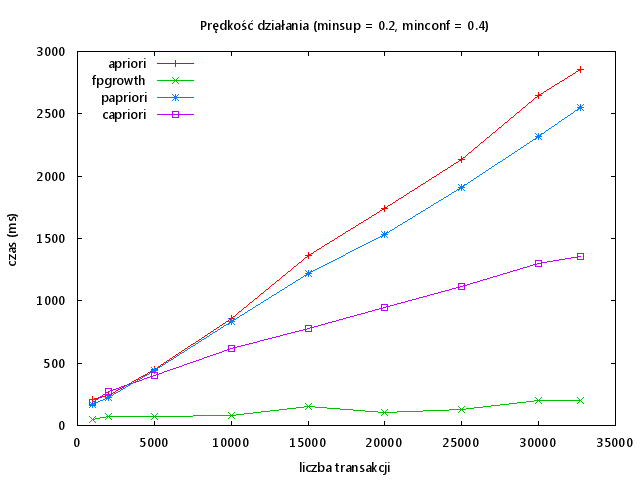
\includegraphics[width=1.1\textwidth]{figures/06/02_04.png}
\caption{Prędkość działania algorytmów\label{rys:02_04}}
\end{figure}

Na rysunku~\ref{rys:02_04} zaprezentowane zostały wyniki działania algorytmów, na podstawie danych zebranych w tablicy~\ref{tab:02_04}. 

Po raz kolejny uwidoczniła się przewaga algorytmu FPGrowth dla danych wejściowych, na których wykonywane były eksperymenty. Algorytm ten przeznaczony jest do danych, których liczności znacząco przekraczały liczbę transakcji w MSWebData.

Hierarchia algorytmów klasy Apriori pozostała nadal taka sama. Najgorzej wypadła klasyczna implementacja, która straciła do ParallelApriori nieco ponad $10\%$, a do CudaApriori niemalże $88\%$. 

ParallelApriori pozostaje bardziej wydajną wersją Apriori, jednakże nadal przegrywa znacząco z CudaApriori - jest on prawie 2 razy wolniejszy od implementacji na karcie graficznej.

\begin{table}
	\centering
	\begin{tabular}{r|r|r|r|r}
	\textbf{l.trans} & \textbf{Apriori} & \textbf{FPGrowth} & \textbf{ParallelApriori} & \textbf{CudaApriori}  \\ \hline
	$1000$ & $211$ & $49$ & $166$ & $185$ \\
	$2000$ & $237$ & $71$ & $221$ & $272$ \\
	$5000$ & $447$ & $72$ & $440$ & $401$ \\
	$10000$ & $857$ & $78$ & $833$ & $617$ \\
	$15000$ & $1367$ & $149$ & $1219$ & $782$ \\
	$20000$ & $1738$ & $106$ & $1534$ & $944$ \\
	$25000$ & $2137$ & $132$ & $1906$ & $1117$ \\
	$30000$ & $2645$ & $200$ & $2321$ & $1299$ \\
	$32711$ & $2856$ & $198$ & $2549$ & $1358$ \\
	\end{tabular}
	\caption{Czasy wykonania poszczególnych algorytmów [ms] (minsup = 0.2, minconf = 0.4)\label{tab:02_04}}
\end{table}

\begin{figure}[H]
\centering
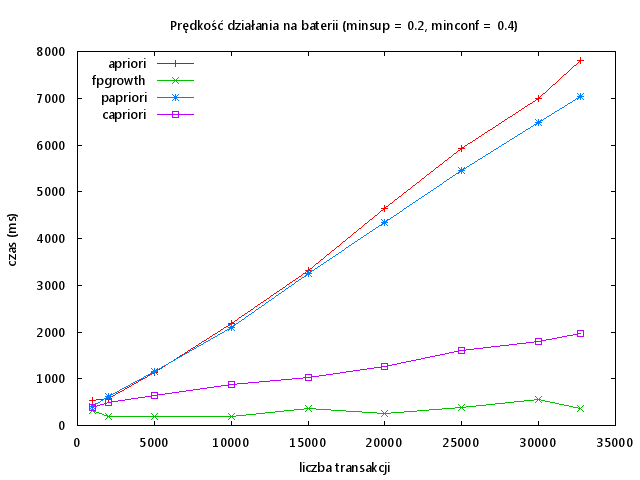
\includegraphics[width=1.1\textwidth]{figures/06/02_04_bat.png}
\caption{Prędkość działania algorytmów na baterii laptopa\label{rys:02_04_bat}}
\end{figure}

Rysunek~\ref{rys:02_04_bat} przedstawia wykres czasów dla tego samego zestawu testów wykonywanego w trybie oszczędzania energii baterii laptopa. Widać znaczący spadek wydajności algorytmów implementowanych na CPU.

Dlatego też spadły wydajności: Apriori, FPGrowth oraz ParallelApriori. Spadała również wydajność CudaApriori, ponieważ (jak wspomniano już wcześniej) część logiki biznesowej została zaimplementowana przy użyciu C\#, a także sama biblioteka CUDA.NET korzysta z CPU. Jednakże spadek wydajności tego algorytmu w porównaniu z pozostałymi jest niemalże pomijalny - wynosi około $30\%$, gdy dla pozostałych (odpowiednio Apriori i ParallelApriori) $174$ i $176\%$.

\begin{table}
	\centering
	\begin{tabular}{r|r|r|r|r}
	\textbf{l.trans} & \textbf{Apriori} & \textbf{FPGrowth} & \textbf{ParallelApriori} & \textbf{CudaApriori}  \\ \hline
	$1000$ & $544$ & $323$ & $407$ & $392$ \\
	$2000$ & $571$ & $194$ & $622$ & $486$ \\
	$5000$ & $1142$ & $190$ & $1151$ & $638$ \\
	$10000$ & $2183$ & $200$ & $2096$ & $881$ \\
	$15000$ & $3324$ & $369$ & $3241$ & $1024$ \\
	$20000$ & $4652$ & $253$ & $4336$ & $1266$ \\
	$25000$ & $5925$ & $378$ & $5446$ & $1596$ \\
	$30000$ & $6996$ & $550$ & $6480$ & $1789$ \\
	$32711$ & $7801$ & $374$ & $7047$ & $1958$ \\
	\end{tabular}
	\caption{Czasy wykonania poszczególnych algorytmów na baterii laptopa [ms] (minsup = 0.2, minconf = 0.4)\label{tab:02_04_bat}}
\end{table}
%%%%%%%%%%%%%%%%%%%%%%%%%%%%%%%%%%%%%%%%%
%%%%%%%%%%%%%%%%%%%%%%%%%%%%%%%%%%%%%%%%%
%%%%%%%%%%%%%%%%%%%%%%%%%%%%%%%%%%%%%%%%%
%%%%%%%%%%%%%%%%%%%%%%%%%%%%%%%%%%%%%%%%%
%%%%%%%%%%%%%%%%%%%%%%%%%%%%%%%%%%%%%%%%%
\subsubsection{Wyniki dla minsup = 0.05, minconf = 0.1}

\begin{figure}[H]
\centering
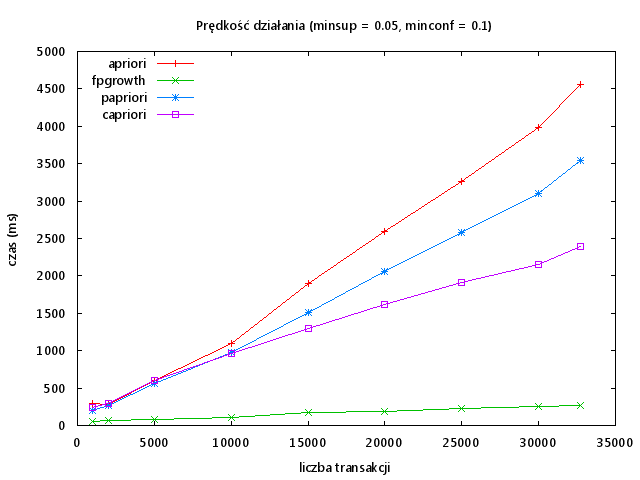
\includegraphics[width=1.1\textwidth]{figures/06/005_01.png}
\caption{Prędkość działania algorytmów\label{rys:005_01}}
\end{figure}

Analizując wykres z rysunku~\ref{rys:005_01} wyraźnie widać wizualizacje, która potwierdza wcześniejsze obserwacje.

W tym wypadku Apriori jest o około $30\%$ wolniejszy od ParallelApriori oraz około $90\%$ wolniejszy od CudaApriori. Przewaga nad algorytmem na karcie graficznej nie jest już tak wyraźna, jak w przypadku poprzednich testów, jednakże nadal jest ona znacząca. 

Algorytm korzystający z PLINQ jest niemal o $50\%$ wolniejszy od wersji na CUDA.

\begin{table}
	\centering
	\begin{tabular}{r|r|r|r|r}
	\textbf{l.trans} & \textbf{Apriori} & \textbf{FPGrowth} & \textbf{ParallelApriori} & \textbf{CudaApriori}  \\ \hline
	$1000$ & $294$ & $60$ & $195$ & $239$ \\
	$2000$ & $280$ & $73$ & $267$ & $294$ \\
	$5000$ & $603$ & $86$ & $560$ & $601$ \\
	$10000$ & $1094$ & $103$ & $970$ & $967$ \\
	$15000$ & $1899$ & $174$ & $1505$ & $1299$ \\
	$20000$ & $2587$ & $193$ & $2053$ & $1619$ \\
	$25000$ & $3266$ & $221$ & $2575$ & $1915$ \\
	$30000$ & $3978$ & $252$ & $3097$ & $2154$ \\
	$32711$ & $4560$ & $273$ & $3546$ & $2392$ \\
	\end{tabular}
	\caption{Czasy wykonania poszczególnych algorytmów [ms] (minsup = 0.05, minconf = 0.1)\label{tab:005_01}}
\end{table}

\begin{figure}[H]
\centering
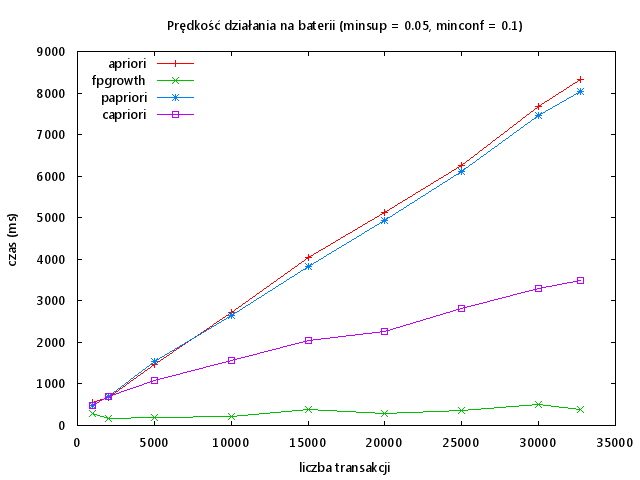
\includegraphics[width=1.1\textwidth]{figures/06/005_01_bat.png}
\caption{Prędkość działania algorytmów na baterii laptopa\label{rys:005_01_bat}}
\end{figure}

Przypadek uruchomienia testów w trybie oszczędnym przedstawia wykres na rysunku~\ref{rys:005_01_bat}, a dane zostały zebrane w tablicy~\ref{tab:005_01_bat}. 

Po raz kolejny można zaobserwować zmniejszenie się różnicy pomiędzy Apriori oraz ParallelApriori, która w tym trybie wyniosła jedynie nieco ponad $3\%$. Powiększyła się strata Apriori oraz ParallelApriori do CudaApriori - wynoszą one odpowiednio $140\%$ oraz $131\%$. 

\begin{table}
	\centering
	\begin{tabular}{r|r|r|r|r}
	\textbf{l.trans} & \textbf{Apriori} & \textbf{FPGrowth} & \textbf{ParallelApriori} & \textbf{CudaApriori}  \\ \hline
	$1000$ & $556$ & $296$ & $481$ & $470$ \\
	$2000$ & $682$ & $167$ & $699$ & $692$ \\
	$5000$ & $1471$ & $203$ & $1534$ & $1085$ \\
	$10000$ & $2719$ & $218$ & $2659$ & $1561$ \\
	$15000$ & $4053$ & $391$ & $3826$ & $2038$ \\
	$20000$ & $5131$ & $284$ & $4931$ & $2269$ \\
	$25000$ & $6248$ & $354$ & $6112$ & $2804$ \\
	$30000$ & $7665$ & $517$ & $7449$ & $3296$ \\
	$32711$ & $8318$ & $393$ & $8045$ & $3480$ \\
	\end{tabular}
	\caption{Czasy wykonania poszczególnych algorytmów na baterii [ms] (minsup = 0.05, minconf = 0.1)\label{tab:005_01_bat}}
\end{table}

%%%%%%%%%%%%%%%%%%%%%%%%%%%%%%%%%%%%%%%%%
%%%%%%%%%%%%%%%%%%%%%%%%%%%%%%%%%%%%%%%%%
%%%%%%%%%%%%%%%%%%%%%%%%%%%%%%%%%%%%%%%%%
%%%%%%%%%%%%%%%%%%%%%%%%%%%%%%%%%%%%%%%%%
%%%%%%%%%%%%%%%%%%%%%%%%%%%%%%%%%%%%%%%%%

\subsubsection{Wyniki dla minsup = 0.05, minconf = 0.4}

\begin{figure}[H]
\centering
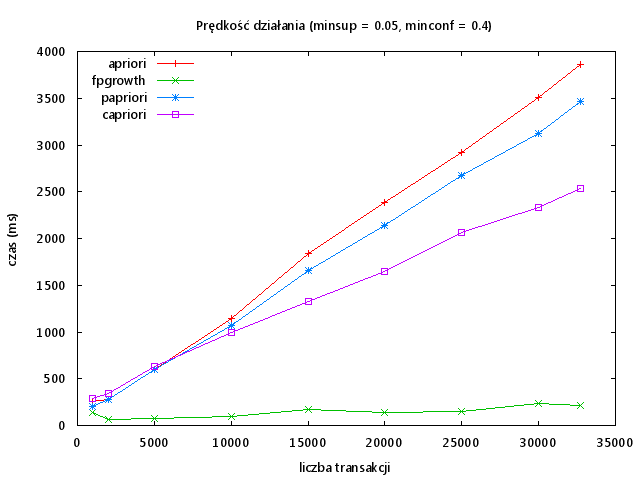
\includegraphics[width=1.1\textwidth]{figures/06/005_04.png}
\caption{Prędkość działania algorytmów\label{rys:005_04}}
\end{figure}

Ostatni z zestawu testów porównawczych dla poszczególnych algorytmów zebrano w tablicy~\ref{tab:005_04} i zaprezentowano na wykresie na rysunku~\ref{rys:005_04}. 

Apriori jest gorszy od ParallelApriori o około $12\%$, a o około $53\%$ gorszy od CudaApriori. Różnica pomiędzy ParallelApriori i CudaApriori jest mniejsza i wynosi $37\%$. 

Po raz kolejny okazało się, że FPGrowth jest najwydajniejszym z zaimplementowanych algorytmów.

\begin{table}
	\centering
	\begin{tabular}{r|r|r|r|r}
	\textbf{l.trans} & \textbf{Apriori} & \textbf{FPGrowth} & \textbf{ParallelApriori} & \textbf{CudaApriori}  \\ \hline
	$1000$ & $256$ & $138$ & $205$ & $286$ \\
	$2000$ & $283$ & $69$ & $276$ & $344$ \\
	$5000$ & $598$ & $78$ & $604$ & $636$ \\
	$10000$ & $1145$ & $91$ & $1073$ & $995$ \\
	$15000$ & $1844$ & $171$ & $1662$ & $1331$ \\
	$20000$ & $2380$ & $141$ & $2138$ & $1647$ \\
	$25000$ & $2922$ & $148$ & $2672$ & $2060$ \\
	$30000$ & $3508$ & $237$ & $3120$ & $2328$ \\
	$32711$ & $3860$ & $212$ & $3464$ & $2531$ \\
	\end{tabular}
	\caption{Czasy wykonania poszczególnych algorytmów [ms] (minsup = 0.05, minconf = 0.4)\label{tab:005_04}}
\end{table}

\begin{figure}[H]
\centering
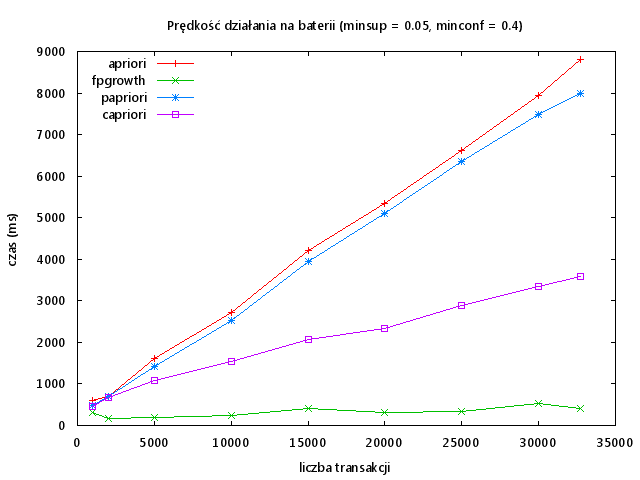
\includegraphics[width=1\textwidth]{figures/06/005_04_bat.png}
\caption{Prędkość działania algorytmów na baterii laptopa\label{rys:005_04_bat}}
\end{figure}

Przypadek testów na baterii, w trybie oszczędzania energii zaprezentowano na rysunku~\ref{rys:005_04_bat} - dane zebrano w tablicy~\ref{tab:005_04_bat}. 

Wyraźnie wzrosły czasy odpowiedzi poszczególnych algorytmów, spowodowane obniżeniem wydajności procesora. Algorytm Apriori jest wolniejszy od CudaApriori o około $146\%$, a jedynie o około $10\%$ od wersji zrównoleglonej przy użyciu PLINQ.

Zaobserwować można również spadek wydajności algorytmu CudaApriori, spowodowany obniżeniem wydajności głównej jednostki komputera, jaką jest procesor.

\begin{table}
	\centering
	\begin{tabular}{r|r|r|r|r}
	\textbf{l.trans} & \textbf{Apriori} & \textbf{FPGrowth} & \textbf{ParallelApriori} & \textbf{CudaApriori}  \\ \hline
	$1000$ & $596$ & $310$ & $483$ & $463$ \\
	$2000$ & $702$ & $177$ & $707$ & $680$ \\
	$5000$ & $1617$ & $197$ & $1421$ & $1086$ \\
	$10000$ & $2719$ & $229$ & $2526$ & $1543$ \\
	$15000$ & $4203$ & $404$ & $3953$ & $2078$ \\
	$20000$ & $5337$ & $322$ & $5102$ & $2328$ \\
	$25000$ & $6606$ & $338$ & $6346$ & $2877$ \\
	$30000$ & $7936$ & $519$ & $7473$ & $3333$ \\
	$32711$ & $8816$ & $407$ & $8000$ & $3582$ \\
	\end{tabular}
	\caption{Czasy wykonania poszczególnych algorytmów na baterii laptopa [ms] (minsup = 0.05, minconf = 0.4)\label{tab:005_04_bat}}
\end{table}

%%%%%%%%%%%%%%%%%%%%%%%%%%%%%%%%%%%%%%%%%
%%%%%%%%%%%%%%%%%%%%%%%%%%%%%%%%%%%%%%%%%
%%%%%%%%%%%%%%%%%%%%%%%%%%%%%%%%%%%%%%%%%
%%%%%%%%%%%%%%%%%%%%%%%%%%%%%%%%%%%%%%%%%
%%%%%%%%%%%%%%%%%%%%%%%%%%%%%%%%%%%%%%%%%

\subsection{Wyniki pomiarów dla algorytmu CudaApriori}

\begin{figure}[H]
\centering
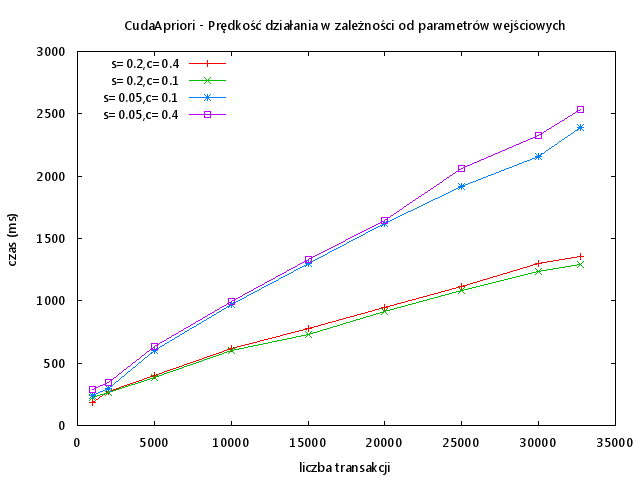
\includegraphics[width=1.1\textwidth]{figures/06/capriori.png}
\caption{Prędkość działania algorytmu CudaApriori w zależności od parametrów wejściowych\label{rys:capriori}}
\end{figure}

\begin{table}
	\centering
	\begin{tabular}{r|r|r|r|r}
	\textbf{l.trans} & \textbf{minsup=0.2} & \textbf{minsup=0.2} & \textbf{minsup=0.05} & \textbf{minsup=0.05}  \\
	 & \textbf{minconf=0.4} & \textbf{minconf=0.1} & \textbf{minconf=0.1} & \textbf{minconf=0.4}  \\ \hline
	$1000$ & $185$ & $221$ & $239$ & $286$ \\
	$2000$ & $272$ & $268$ & $294$ & $344$ \\
	$5000$ & $401$ & $388$ & $601$ & $636$ \\
	$10000$ & $617$ & $601$ & $967$ & $995$ \\
	$15000$ & $782$ & $726$ & $1299$ & $1331$ \\
	$20000$ & $944$ & $914$ & $1619$ & $1647$ \\
	$25000$ & $1117$ & $1080$ & $1915$ & $2060$ \\
	$30000$ & $1299$ & $1232$ & $2154$ & $2328$ \\
	$32711$ & $1358$ & $1291$ & $2392$ & $2531$ \\
	\end{tabular}
	\caption{Czasy wykonania algorytmu CudaApriori w zależności od parametrów wejściowych [ms]\label{tab:capriori}}
\end{table}

Rysunek~\ref{rys:capriori} prezentuje zebrane wyniki wykonania algorytmu CudaApriori w zależności od parametrów wejściowych. Tablica~\ref{tab:capriori} zawiera czasy, które były podstawą wykonania wykresu. Wyniki dla poszczególnych parametrów został omówione wcześniej. 

Z wykresu można wyciągnąć bardzo interesujące wnioski. Wyraźnie widać, że wykresy są liniowe z różnym współczynnikiem nachylenia prostej do osi X - podział taki można zrobić na dwie grupy wykresów. Z jednej strony mamy wykresy dla parametrów minsup=$0.2$, minconf=$0.4$ oraz minsup=$0.2$, minconf=$0.1$, które to są pochylone pod mniejszym kontem niż wykresy minsup=$0.05$, minconf=$0.4$ i minsup=$0.05$, minconf=$0.1$. 

Powyższa obserwacja prowadzi do wniosku, że wartość parametru $minsup$ wpływa wprostproporcjonalnie na czas obliczeń algorytmu. W rodziale~\ref{chap:algorytm} opisano algorytm CudaApriori, w którym przedstawiono wpływ $minsup$ na algorytm. Wynika z tego jasno, że im wyższa wartość tego parametru, tym mniej zbiorów jest generowanych w $L_1$, a także w kolejnym kroku mniejsza jest liczebność zbiorów $L_k$. Dlatego też im wyższa jest wartość $minsup$, tym krótszy jest czas obliczeń, ponieważ mniejsza jest liczba zbiorów poddawana procedurze generowania kandydatów i tak dalej. Różnice pomiędzy wykonaniami z tymi samymi wartościami $minconf$ ($minconf$ odpowiednio $0.4$ i $0.1$) $85\%$ i $86\%$.

Poza zależnością wynikającą z parametru $minsup$ pozostaje jeszcze kwestia różnic spowodowanych parametrem $minconf$. Dzieląc wykonane testy na dwie grupy (odpowiednio dla $minsup=0.2$ oraz $minsup=0.05$) uwidacznia się krótszy czas wykonywania obliczeń dla niższej wartości $minconf$. Różnice pomiędzy algorytmami wynoszą $5\%$ oraz około $5,5\%$. 

\begin{figure}[H]
\centering
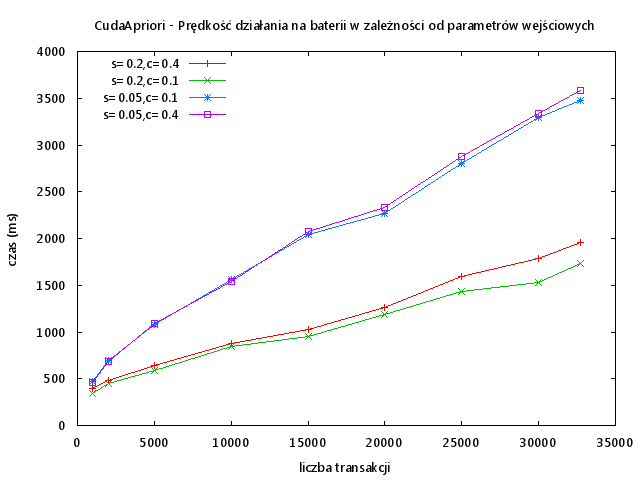
\includegraphics[width=1.1\textwidth]{figures/06/capriori_bat.png}
\caption{Prędkość działania algorytmu CudaApriori na baterii laptopa w zależności od parametrów wejściowych\label{rys:capriori_bat}}
\end{figure}

\begin{table}
	\centering
	\begin{tabular}{r|r|r|r|r}
	\textbf{l.trans} & \textbf{minsup=0.2} & \textbf{minsup=0.2} & \textbf{minsup=0.05} & \textbf{minsup=0.05}  \\
	 & \textbf{minconf=0.4} & \textbf{minconf=0.1} & \textbf{minconf=0.1} & \textbf{minconf=0.4}  \\ \hline
	$1000$ & $392$ & $339$ & $470$ & $463$ \\
	$2000$ & $486$ & $445$ & $692$ & $680$ \\
	$5000$ & $638$ & $592$ & $1085$ & $1086$ \\
	$10000$ & $881$ & $847$ & $1561$ & $1543$ \\
	$15000$ & $1024$ & $951$ & $2038$ & $2078$ \\
	$20000$ & $1266$ & $1183$ & $2269$ & $2328$ \\
	$25000$ & $1596$ & $1436$ & $2804$ & $2877$ \\
	$30000$ & $1789$ & $1527$ & $3296$ & $3333$ \\
	$32711$ & $1958$ & $1734$ & $3480$ & $3582$ \\
	\end{tabular}
	\caption{Czasy wykonania algorytmu CudaApriori na baterii laptopa w zależności od parametrów wejściowych [ms]\label{tab:capriori_bat}}
\end{table}

Podobnie, jak wypadku testów wyniki dla uruchomień na baterii wyznaczają podobne trendy - widoczne na wykresie na rysunku~\ref{rys:capriori_bat}.

Różnice dla wyników eksperymentów z tym samym $minconf$ wynoszą $100$ i $82\%$. Widać, że różnica w porównaniu z uruchomieniem na pełnej wydajności zwiększyła się. Widać, że dla większej liczby operacji (wynikającej bezpośrednio z większej liczby zbiorów częstych) większa też jest logika biznesowa, która wykonywana była na CPU. Z tego właśnie wynika fakt większych (choć nieznacznie) różnic pomiędzy algorytmami. 

Dla stałego parametru $minsup$ różnice $13\%$ i $3\%$. Jak widać różnice pozostały na podobnym poziomie. Widać, że dla $minsup=0.2$ wzrosła różnica w porównaniu do testów na pełnej mocy procesora.

\section{Podsumowanie eksperymentów i wnioski}

Warto zauważyć, że algorytm CudaApriori okazał się znacząco szybszy od pozostałych algorytmów z tej klasy (tzw. \emph{apriori-like}) zaimplementowane na potrzeby niniejszej pracy. Porównanie z FPGrowth wykazało jego nadal niską wydajność w porównaniu z innymi algorytmami o mniejszej złożoności. 

Zaprezentowana i opisana została wydajność algorytmu w szeregu testów, szczegółowo opisanych w poszczególnych sekcjach niniejszego rozdziału. Przedstawiono również analizę wydajności algorytmu CudaApriori w zależności od parametrów wejściowych do algorytmu. Wynika z tego, że podczas uruchamiania testów na systemach, w których potrzebna jest szybka odpowiedź bardzo ważnym elementem analizy jest umiejętne dobranie parametrów algorytmu.